\section{Tecnolog\'ia a Utilizar}
\label{sec:tecnologia-utilizada}

\subsection{TamTam Edit}

La aplicaci\'on que se ha elegido para este trabajo de grado consiste en una
Actividad\footnote{Una Actividad, es una aplicaci\'on en el entorno de escritorio \emph{Sugar}}
musical para la
computadora
XO,\footnote{La XO, es una computadora port\'atil de bajo costo y consumo desarrollada por el proyecto \emph{One Laptop Per Child}}denominada \emph{TamTam Edit}.

\emph{TamTam Edit} es una aplicaci\'on, que forma parte del conjunto de actividades musicales \emph{TamTam}, que proporciona
una interfaz intuitiva para crear, modificar y organizar notas ubicadas en pistas virtuales. Adem\'as incluye una paleta de
casi cien tipos de sonidos y modelos de construcci\'on musical que permite crear distintos tipos de variaciones en estilos
musicales \cite{TamTamWiki}.

Las secciones principales del programa se pueden observar en la figura~\ref{figure:ui-tamtam} 

\begin{figure}[H]
\centering
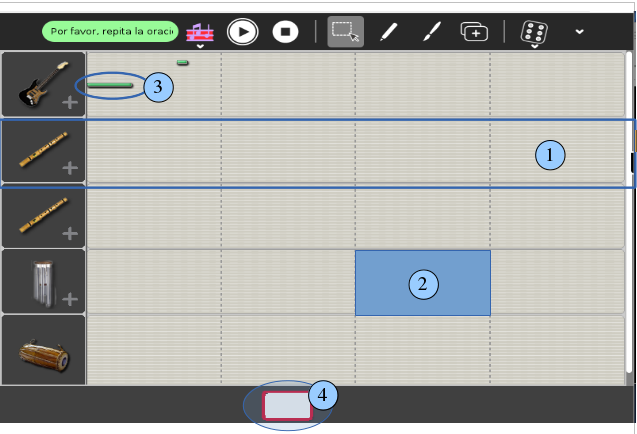
\includegraphics[width=\textwidth]{./graphics/ui-tamtam-edit.png}
\caption{Interfaz de \emph{Tamtam Edit} y sus secciones principales}
\label{figure:ui-tamtam}
\end{figure}

Como se puede apreciar, la interfaz se encuentra organizada en cinco pistas y cada pista tiene asociada un 
instrumento (la quinta pista esta reservada para instrumento de tipo batería). Cada pista se divide en 4 
compases (del compás uno al cuatro) y cada compás se divide en 12 tiempos (del uno al doce). 
Las notas se dibujan en los compases, como se puede ver, la longitud de la nota indica su duración y su 
altura el tipo de nota. Además la aplicación esta organizada en partituras, que son como hojas de 
cuaderno, y son útiles para componer músicas largas.

A continuaci\'on se presentan los motivos que determinaron la elecci\'on de esta aplicaci\'on:

\begin{itemize}
    \item \emph{Impacto social:} \emph{TamTam Edit} es una aplicaci\'on que forma parte de una plataforma establecida
    por el proyecto \gls{olpc}. Este proyecto busca proveer
	a cada ni\~no de pa\'ises en desarrollo de una computadora de bajo costo con el
	fin de potenciar el proceso educativo \cite{OLPC}. Ni\~nos con alg\'un tipo de discapacidad podr\'ian tener
	problemas para utilizar la computadora. Por ejemplo, un ni\~no con problemas motrices podr\'ia tener dificultades para operar el mouse
	o el teclado. Para estos casos, operar esta actividad utilizando la voz beneficiar\'ia a los ni\~nos con discapacidades
	y por lo tanto la aplicaci\'on tendr\'ia un impacto social positivo, debido a la mejora en la accesibilidad.
    \item \emph{Naturalidad de interacci\'on:} utilizar la voz para interactuar con una aplicaci\'on presenta una mayor
	naturalidad con respecto al enfoque tradicional de interacci\'on, debido a que es el medio de
	interacci\'on entre las personas.
    \item \emph{No reinventar la rueda:} como el objetivo es incorporar una interfaz basada en reconocimiento del habla a una aplicaci\'on,
	se elige \emph{TamTam Edit} para no construir la aplicaci\'on desde cero, sino extender las capacidades de una ya existente.
    \item \emph{C\'odigo abierto:} el motivo anterior es posible gracias a que \emph{TamTam Edit} es un proyecto de c\'odigo abierto, lo cual
	brinda a los desarrolladores la libertad de extender las funcionalidades de la aplicaci\'on.
    \item \emph{Lenguaje de programaci\'on:} la actividad se encuentra implementada en el lenguaje de programaci\'on Python. Este es el
	lenguaje elegido para realizar la interfaz, adem\'as la librer'ia de reconocimiento del habla a ser utilizada proporciona
	\emph{bindings} para este lenguaje.
\end{itemize}



\subsection{PocketSphinx}

Para la implementaci\'on de la interfaz operable a trav\'es de la voz se ha elegido la librer\'ia \emph{PocketSphinx} que,
como se menciona en la secci\'on \ref{sec:pocketsphinx}, es un motor de reconocimiento del habla orientado a la optimaci\'on
del rendimiento y la portabilidad.

Uno de los objetivos espec\'ificos de este trabajo de grado es aplicar y contrastar en la pr\'actica
los conocimientos te\'oricos adquiridos. Como indica la secci\'on \ref{sec:librerias}, una librer\'ia es
el tipo de herramienta que requiere un conocimiento t\'ecnico espec\'ifico del \'area, adem\'as de
brindar una alta flexibilidad permitiendo al programador manipular los distintos componentes del
proceso de reconocimiento del habla. Por lo tanto una librer\'ia es la herramienta m\'as adecuada
para cumplir el objetivo mencionado anteriormente.

A continuaci\'on se presentan los motivos t\'ecnicos que determinaron la elecci\'on de esta librer\'ia:

\begin{itemize}
    \item Existen \foreign{bindings} para el lenguaje de programaci\'on Python, lo cual hace muy sencilla la tarea de utilizar
	la librer\'ia desde el c\'odigo Python.
    \item \emph{PocketSphinx} esta orientada a la optimizaci\'on del rendimiento, resultando adecuada para sistemas con
	recursos limitados, como es el caso de la computadora \emph{XO}.
    \item La librer\'ia es un proyecto de c\'odigo abierto, por lo tanto se cumple la metodolog\'ia de trabajo que se ha
	establecido para este trabajo de grado: utilizar herramientas de c\'odigo abierto para la implementaci\'on de la
	interfaz.
\end{itemize}
